\newpage
%
% Návrh
%
\ifthenelse {\boolean{bachelor}}
{
	%\section{Design}
	\section{Návrh}
}
{
	%\chapter{Design}
	\chapter{Návrh}
}
\label{section:design}

%
% Návrh uchovávania textov v databázach
%
\ifthenelse {\boolean{bachelor}}
{
	%\subsection{Subsection}
	\subsection{Návrh uchovávania textov v databázach}
}
{
	%\section{Subsection}
	\section{Návrh uchovávania textov v databázach}
}
\label{subsection:our_design_persisting_data}
Na uchovávanie dát sme zvolili dokumentovú databázu MongoDB. Ukladané dáta sa dajú rozdeliť do niekoľkých samostatných kolekcií. Sú to:

\begin{my_itemize}
	\myitem rules,
	\myitem sentences,
	\myitem notes
	\myitem structures,
	\myitem articles,
	\myitem and rules.
\end{my_itemize}
	
Prepojenia medzi jednotlivými kolekciami sú zobrazené na obrázku~\fullref{fig:db_schema}. Nasledujúcich časti opisujú stručne každú kolekciu. Všetky kolekcie obsahujú okrem polí špecifických pre danú kolekciu, aj polia časových značiek označujúcich vytvorenie a aktualizáciu záznamu.

\begin{figure}[H]
	\begin{center}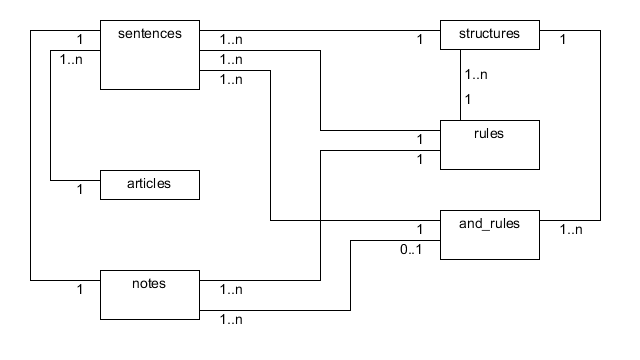
\includegraphics[scale=0.60]{db_schema}\end{center}
	\caption[Databázový model]{Databázový model}\label{fig:db_schema}
\end{figure}

%
% Kolekcia texts
%
\ifthenelse {\boolean{bachelor}}
{
	%\subsection{Subsection}
	\subsubsection{Kolekcia articles}
}
{
	%\section{Subsection}
	\subsection{Kolekcia articles}
}
\label{subsubsection:collection_articles}
V kolekcií \textit{articles} sa ukladajú spracovávané texty. 

Kolekcia obsahuje textové pole \textit{text} na uloženie textu v pôvodnom tvare. Model kolekcie \textit{articles} je zobrazený na obrázku~\fullref{fig:articles_collection_model}.

\begin{figure}[H]
	\begin{center}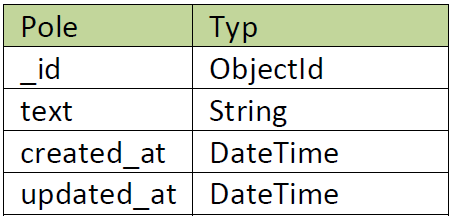
\includegraphics[scale=0.60]{articles_model}\end{center}
	\caption[Model kolekcie articles]{Model kolekcie articles}\label{fig:articles_collection_model}
\end{figure}

%
% Kolekcia notes
%
\ifthenelse {\boolean{bachelor}}
{
	%\subsection{Subsection}
	\subsubsection{Kolekcia notes}
}
{
	%\section{Subsection}
	\subsection{Kolekcia notes}
}
\label{subsubsection:collection_notes}
Kolekcia \textit{notes} uchováva vytvorené poznámky z viet.

Obsahuje textové pole \textit{text} s hodnotou poznámky a dve referencujúce polia. Jedno sa odkazuje do kolekcie \textit{rules} na pravidlo, ktoré bolo použité na vytvorenie poznámky. Druhé referencuje použité and\hyph pravidlo v kolekcií \textit{and\textunderscore rules}. Toto pole môže byť prázdne, ak sa and\hyph pravidlo pri vytváraní poznámky nepoužilo. Na obrázku~\fullref{fig:notes_collection_model} je vyobrazený model kolekcie \textit{notes}.

\begin{figure}[H]
	\begin{center}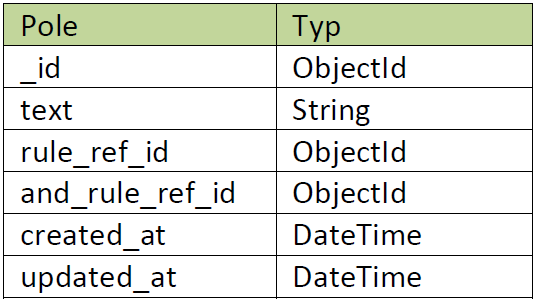
\includegraphics[scale=0.60]{notes_model}\end{center}
	\caption[Model kolekcie notes]{Model kolekcie notes}\label{fig:notes_collection_model}
\end{figure}

%
% Kolekcia sentences
%
\ifthenelse {\boolean{bachelor}}
{
	%\subsection{Subsection}
	\subsubsection{Kolekcia sentences}
}
{
	%\section{Subsection}
	\subsection{Kolekcia sentences}
}
\label{subsubsection:collection_sentences}
V následujúcej kolekcií \textit{sentences} sa ukladajú spracované vety aj s informáciami o článku, pravidlách a poznámke.

Kolekcia sa skladá z textového polia \textit{text} uchovávajúce hodnotu vety a piatich referencujúcich polí \textit{article\textunderscore ref\textunderscore id}, \textit{structure\textunderscore ref\textunderscore id}, \textit{rule\textunderscore id}, \textit{rule\textunderscore ref\textunderscore id}, \textit{and \textunderscore rule\textunderscore ref\textunderscore id} a \textit{note\textunderscore id}. \textit{Article\textunderscore ref\textunderscore id} odkazuje na článok z kolekcie \textit{articles}, ktorého súčasťou je daná veta. Pole \textit{structure\textunderscore ref\textunderscore id} odkazuje do kolekcie \textit{structures}, ktoré reprezentuje štruktúru vety. Nasledujúce polia \textit{rule\textunderscore ref\textunderscore id} a \textit{and\textunderscore rule\textunderscore ref\textunderscore id} odkazujú na použité pravidlo a and\hyph pravidlo pri spracovávaní vety, v tomto poradí. Pole \textit{note\textunderscore ref\textunderscore id} odkazuje na poznámku z kolekcie \textit{notes}, ktorá bola vytvorená z vety.

Model tejto kolekcie je načrtnutý na obrázku~\fullref{fig:sentences_collection_model}.

\begin{figure}[H]
	\begin{center}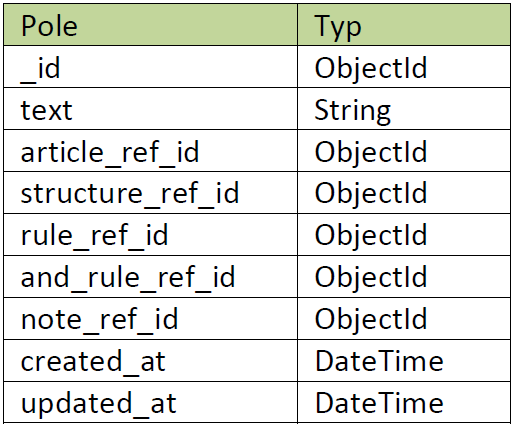
\includegraphics[scale=0.60]{sentences_model}\end{center}
	\caption[Model kolekcie sentences]{Model kolekcie sentences}\label{fig:sentences_collection_model}
\end{figure}

%
% Kolekcia structures
%
\ifthenelse {\boolean{bachelor}}
{
	%\subsection{Subsection}
	\subsubsection{Kolekcia structures}
}
{
	%\section{Subsection}
	\subsection{Kolekcia structures}
}
\label{subsubsection:collection_structures}
V kolekcií \textit{structures} sú uložené štruktúry viet a pravidiel. Štruktúra je zložená hlavne zo závislostí, tokenov, názvoslovných značiek, indexov a iné.

Kolekcia sa skladá z jedného pola \textit{structure\textunderscore data}. Toto pole je zoznam dokumentov, obsahujúcich vyššie spomenuté údaje. Dokument v tomto zozname obsahuje textové pole \textit{dependency\textunderscore name} s názvom závislosti a zoznam dokumentov závislostí \textit{dependencies} s týmto názvom. Dokument v zozname \textit{dependencies} sa skladá z polí \textit{governor} a \textit{dependent} typu dokument, celočíselného pola \textit{position} uchovávajúceho pozíciu závislosti vo vete alebo poznámke, \textit{comparison\textunderscore type}, ktoré je celočíselnou reprezentáciou typu porovnania a poľa \textit{token\textunderscore type}, ktoré je taktiež celočíselnou reprezentáciou typu tokenu. Dokumenty polí \textit{governor} a \textit{depdendent} obsahujú údaje o prislúchajúcich tokenoch závislosti. V textovom poli \textit{POS} sa ukladá značka slovného druhu, pole \textit{index} uchováva index tokenu vo vete, \textit{ner} je textové pole reprezentujúce názvoslovnú entitu tokenu a v poli \textit{lemma} je textová reprezentácia lemy tokenu.

Celý model kolekcie je zobrazený na obrázku~\fullref{fig:structures_collection_model}.

\begin{figure}[H]
	\begin{center}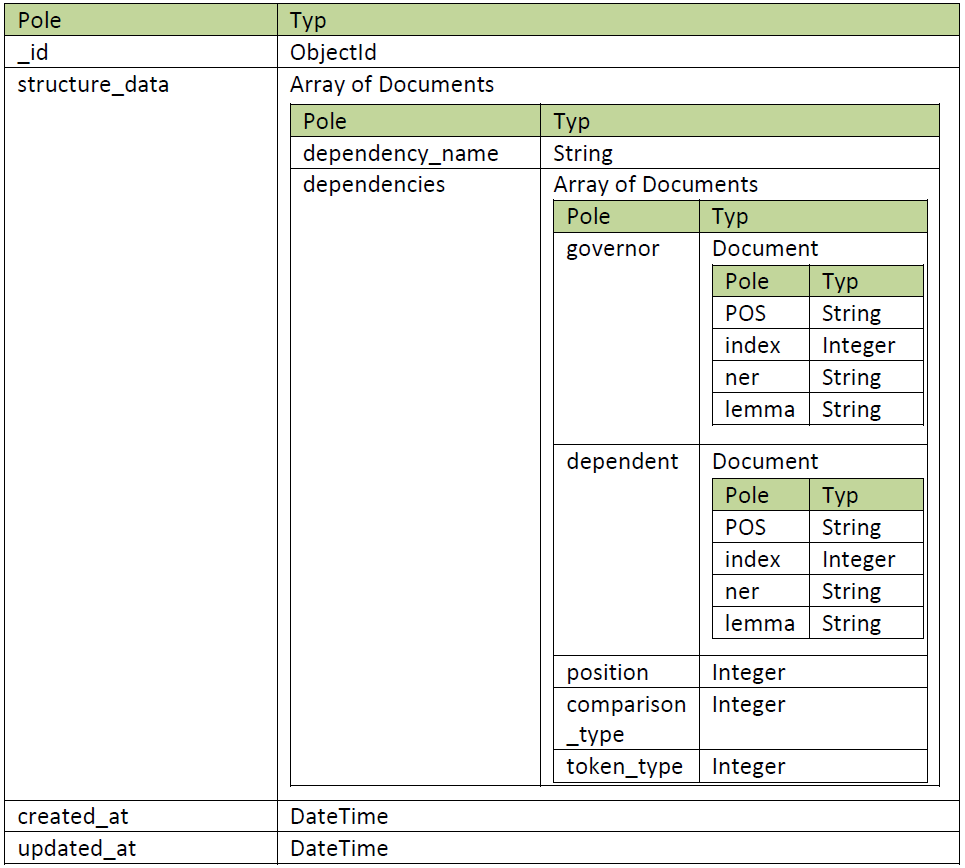
\includegraphics[scale=0.53]{structure_model}\end{center}
	\caption[Model kolekcie structures]{Model kolekcie structures}\label{fig:structures_collection_model}
\end{figure}

%
% Kolekcia rules
%
\ifthenelse {\boolean{bachelor}}
{
	%\subsection{Subsection}
	\subsubsection{Kolekcia rules}
}
{
	%\section{Subsection}
	\subsection{Kolekcia rules}
}
\label{subsubsection:collection_rules}
\textit{Rules} je kolekcia, do ktorej sa ukladajú pravidla na vytvorenie poznámok z viet. Vďaka databázovému modelu na obrázku~\fullref{fig:db_schema} a prepojeniam medzi kolekciami je táto kolekcia minimalistická.

Skladá sa z dvoch polí. Pole \textit{sentence\textunderscore terminators} je zoznam čísel, ktoré reprezentujú konce viet v poznámke. Referencujúce pole \textit{structure\textunderscore ref\textunderscore id} odkazuje do kolekcie \textit{structures} na štruktúru, ktorou sa má prípadná veta spracovať. Model kolekcie \textit{rules} je vyjadrený obrázkom~\fullref{fig:rules_collection_model}.

Pole \textit{sentence\textunderscore terminators} zväčša obsahuje jeden záznam. Napríklad pri vete \textit{,,The president of the Slovak Republic is andrej Kiska.''} a poznámke z tejto vety v tvare \textit{,,President is Kiska.''} bude obsahovať jeden záznam: 3. Číslo 3 preto, lebo koniec vety, v tomto prípade bodka, sa nachádza na tretej pozícií spomedzi tokenov vo vete. Číslovanie pozícií začína indexom nula. V prípade ak veta je súvetie, zložené z viacerých jednoduchých viet, môže pole \textit{sentence\textunderscore terminators} obsahovať viacero záznamov, ak napríklad chceme z každej jednoduchej vety súvetia získať zjednodušenú vetu a vytvoriť tak zloženú poznámku, skladajúcu sa zo zjednodušených viet.

\begin{figure}[H]
	\begin{center}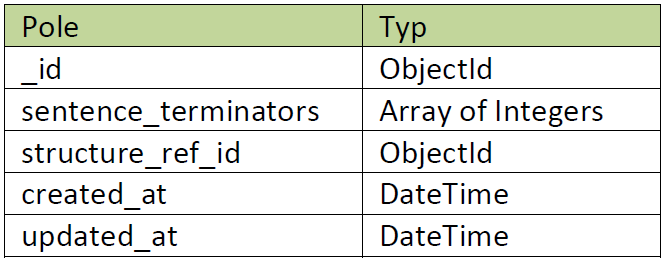
\includegraphics[scale=0.60]{rules_model}\end{center}
	\caption[Model kolekcie rules]{Model kolekcie rules}\label{fig:rules_collection_model}
\end{figure}

%
% Kolekcia and_rules
%
\ifthenelse {\boolean{bachelor}}
{
	%\subsection{Subsection}
	\subsubsection{Kolekcia and rules}
}
{
	%\section{Subsection}
	\subsection{Kolekcia and rules}
}
\label{subsubsection:collection_and_rules}
Posledná kolekcia uchováva pravidlá pre spracovanie vety a vytvorenie viacnásobnej poznámky z vety. Táto kolekcia je veľmi podobná kolekcií \textit{rules} a obsahuje rovnaké polia doplnené o ďalšie špecifické pole.

Špecifické pole, o ktoré je kolekcia rozšírená oproti kolekcií \textit{rules} je celočíselné pole \textit{set\textunderscore position}. Toto pole uchováva pozíciu množiny v viacnásobnej poznámke. Model kolekcie je vyobrazený na obrázku~\fullref{fig:and_rules_collection_model}.

\begin{figure}[H]
	\begin{center}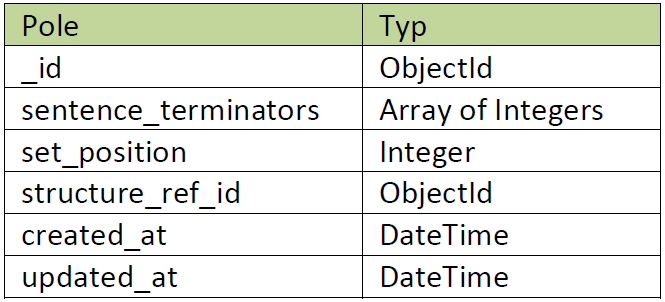
\includegraphics[scale=0.60]{and_rules_model}\end{center}
	\caption[Model kolekcie and rules]{Model kolekcie and rules}\label{fig:and_rules_collection_model}
\end{figure}

%Dáta sú v MongoDB databáze uložené v binárnom JSON formáte. Na ukážke~\fullref{code:collection_rules_data_example} je zobrazená časť uložených údajov o pôvodnej vete. Ukážka celého záznamu pre vetu ,,The president of the Czech Republic is Milos Zeman.'' je priložená v prílohe~\fullref{appendix:db_entry_full_example}.
%\\
%\begin{lstlisting}[language = json, caption={Ukážka dát kolekcie rules}, label = {code:collection_rules_data_example}]
%{  
%	"originalDependencies" : [  
%		{  
%			"dependencyName" : "det",
%			"dependencies" : [  
%				{  
%					"governor" : {  
%						"pos" : "NN",
%						"index" : 2
%					},
%					"dependent" : {  
%						"pos" : "DT",
%						"index" : 1
%					},
%					"position" : 0
%				},
%				{ ... }
%			]
%		}
%	]
%}
%\end{lstlisting}

%
% Kolekcie zhrnutie
%
\ifthenelse {\boolean{bachelor}}
{
	%\subsection{Subsection}
	\subsubsection{Zhrnutie}
}
{
	%\section{Subsection}
	\subsection{Zhrnutie}
}
\label{subsubsection:collections_summary}
Pri návrhu databázového modelu a kolekcií sme vychádzali z princípu jednoduchých kolekcií so zoskupením súvisiacich dát a oddelenia ich od zvyšku. Vďaka využívaniu viacerých, medzi sebou prepojených, kolekcií sme zabezpečili neduplikovanie dát, jednoduché vyhľadanie napríklad viet ku článku a iné. Okrem toho nám tento model umožňuje ďalšiu funkcionalitu, ako napríklad aplikovanie jedného pravidla na viacero viet so zhodnou štruktúrou. Oddelenie dát do samostatných štruktúr nám uľahčuje aj prípadne neskoršie rozšírenie databázového modelu alebo zmenu konkrétnych štruktúr. Taktiež uľahčuje prípadné klastrovanie databázy, ak by bolo nutné, keďže každá kolekcia by mohla byť na samostatnom serveri.


%
% Manažment dát
%
\ifthenelse {\boolean{bachelor}}
{
	%\subsection{Subsection}
	\subsection{Manažment dát}
}
{
	%\section{Subsection}
	\section{Manažment dát}
}
\label{subsection:data_management}
V nasledujúcich častiach si priblížime prácu s dátami z databázy, ako vyhľadanie pravidla, jeho aplikovanie alebo vytvorenie pravidla, ak žiadne nebolo vyhľadané.

%
% Vyhľadávanie pravidla
%
\ifthenelse {\boolean{bachelor}}
{
	%\subsection{Subsection}
	\subsubsection{Vyhľadanie pravidla}
}
{
	%\section{Subsection}
	\subsection{Vyhľadanie pravidla}
}

\label{subsubsection:rule_lookup}
Pri spracovávaní vety, pred vytvorením poznámky, aplikovateľné pravidlo musí byť vyhľadané v databáze. Závislosti pravidla a závislostí vety musia spolu korešpondovať. Pre vyhľadanie pravidla, pravidlo aj veta musia obsahovať rovnakú množinu závislostí. To znamená mať rovnaký počet záznamov v \textit{zozname dát o pôvodnej vete} a zároveň tieto záznamy musia obsahovať rovnaké názvy vzťahov závislostí.

Aplikovateľné pravidlo je vyhľadané ak hlavná podmienka je splnená. Avšak, táto podmienka môže spôsobiť, že viacero aplikovateľných pravidiel je vyhľadaných. V takom prípade zhoda spracovávanej vety a originálnej vety obdržanej z pravidla musí byť vypočítaná. Pravidlo s najväčšou zhodou je následne aplikované.

Výpočet zhody pozostáva z niekoľkých krokov. Najskôr je separátne vypočítaná zhoda POS značiek podradeného a nadradeného tokenu. Indexy nadradeného a podradeného tokenu su taktiež vypočítané separátne. Tieto prvé kroky určia, či veta obsahuje ľubovolnú závislosť s rovnakou POS značkou alebo indexom. V nasledujúcom kroku je určená polovičná zhoda závislostí. Polovičná zhoda závislosti je zhoda POS značky a indexu nadradeného alebo podradeného tokenu. Zhodu POS značky a indexu nadradeného alebo podradeného tokenu počítame pre každú závislosť. Nakoniec, v poslednom kroku, počítame počet úplne zhodných závislostí. Úplní zhoda závislosti je zhoda POS značky a indexu nadradeného, a zároveň podradeného tokenu. Každý krok ma priradené ohodnotenie. Ak je podmienka v kroku vyhodnotená ako správna, ohodnotenie kroku je pripočítané do finálnej hodnoty. Finálna zhoda je percentuálne ohodnotenie zhody. Ohodnotenie krokov odzrkadľuje dôležitosť daného kroku vo výpočte presnej zhody, pričom závisí od počtu závislostí a krokov, takže finálna zhoda nemôže presiahnuť hodnotu 100\%. Pseudokód~\ref{alg:calculating_match} zobrazuje algoritmus výpočtu zhody, konkrétny príklad je zobrazený na obrázku~\fullref{fig:calculate_match_sentences_example}

\begin{algorithm}[H]
	\floatname{algorithm}{Algoritmus}
	\footnotesize %\small, \footnotesize, \scriptsize, or \tiny
	\begin{algorithmic}[1]

		\Procedure{CalculateMatch}{$sentence, originalDependencies$}
		\State $oneCompareTypeRating \gets \text{calculate percentage rating of one comparison}$
		
		\ForAll {$originalDependencies$}
		\If {$\text{count(}sentence\text{, }dependency\text{) =  count(}originalDependencies\text{, }dependency\text{)}$}
		\State $match \gets match \text{ + } oneCompareTypeRating$
		\EndIf
		\State $counter \gets counter \text{ + } \text{count(}originalDependencies\text{, } dependency\text{)}$
		\EndFor
		
		\State $oneCompareTypeRating \gets oneCompareType / counter$
		\ForAll {$originalDependency$}
		\ForAll {$dependency$}
		\ForAll {$comparison$}
		\If {$\text{applyComparison(}sentence, comparison, dependency\text{)}$}
		\State $match \gets match \text{ + } oneCompareTypeRating$
		\EndIf
		\EndFor
		\EndFor
		\EndFor
		
		\Return $match$
		\EndProcedure
	\end{algorithmic}
	\caption[Výpočet zhody]{Výpočet zhody}	
	\label{alg:calculating_match}
\end{algorithm}

\begin{figure}[H]
	\begin{center}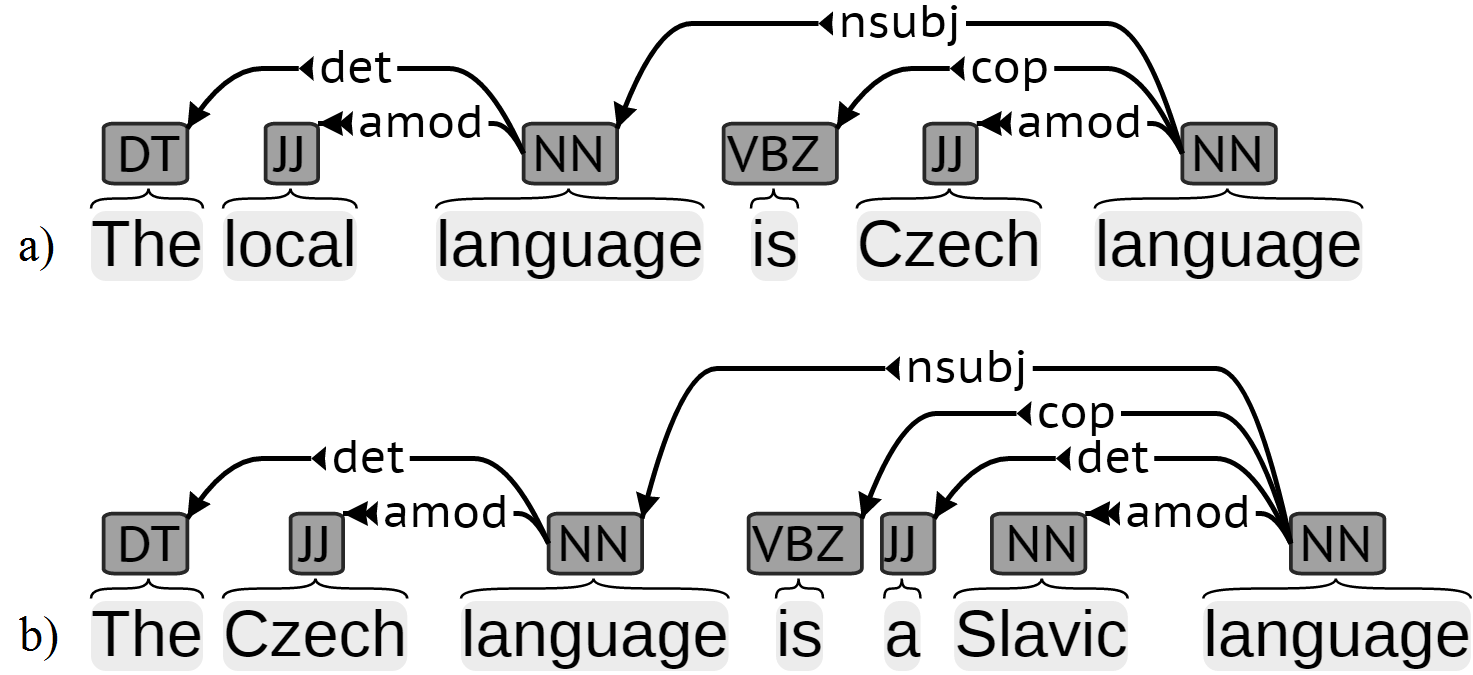
\includegraphics[scale=0.2]{calculate_match_sentences_example}\end{center}
	\caption[Príklad určenia zhody]{Príklad určenia zhody}\label{fig:calculate_match_sentences_example}
\end{figure}

Predpokladajme situáciu z obrázka~\fullref{fig:calculate_match_sentences_example}. Máme pravidlá pre dve vety s spracovávame prvú z nich. V tejto situácií, minimálne dve pravidlá su aplikovateľné na vetu \textit{a}. Predpokladajme, že vypočítavame zhodu s vetou \textit{b}. Prechádzame postupne cez všetky závislosti spracovávanej vety \textit{a}. Prvá závislosť je so vzťahom \textit{det}, nadradeným tokenom s POS značkou NN (noun - podstatné meno) a indexom 3 a podradeným tokenom s POS značkou DT (determiner - determinant) a indexom 1. V prvok kroku zistíme, či veta \textit{b} obsahuje závislosť so vzťahom \textit{det} a tokenmi s POS značkami NN alebo DT and indexmi rovnými 1 alebo 3. Toto je separátny výpočet POS značiek a indexov. v nasledujúcom kroku zisťujeme, či veta \textit{b} obsahuje závislosť so vzťahom \textit{det} a nadradeným alebo podradeným tokenom s POS značkou NN a indexom 3 alebo POS značkou DT a indexom 1. Toto je polovičná zhoda. V poslednom kroku hľadáme vo vete \textit{b} závislosť so vzťahom \textit{det} a nadradeným tokenom práve s POS značkou NN a indexom 3 a zároveň podradený token práve s POS značkou DT a indexom 1. Ak ktorýkoľvek krok bol vyhodnotený ako správny, jeho ohodnotenie je pridané ku koncovému výsledku a iterácia pokračuje s nasledujúcou závislosťou, pokým sa nevyhodnotí posledná.

Aplikovaním určenia zhody vety \textit{a} s vetami \textit{a} a \textit{b} zistíme, že s vetou \textit{a} má zhodu $100\%$ a s vetou \textit{b} má cca. $63,57\%$ zhodu.

%\begin{figure}[H]
%	\begin{center}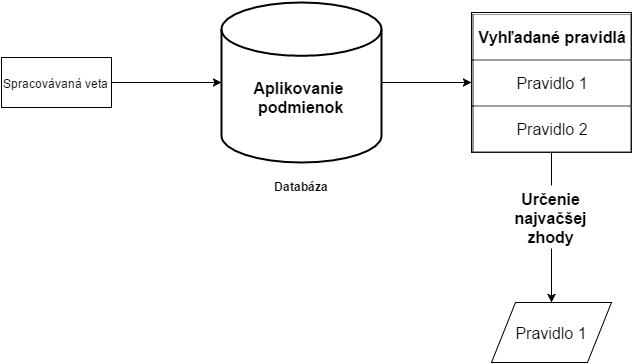
\includegraphics[scale=0.6]{rule_lookup}\end{center}
%	\caption[Vyhľadanie pravidla]{Vyhľadanie pravidla}\label{fig:rule_lookup}
%\end{figure}

%
% Aplikovanie pravidla
%
\ifthenelse {\boolean{bachelor}}
{
	%\subsection{Subsection}
	\subsubsection{Aplikovanie pravidla}
}
{
	%\section{Subsection}
	\subsection{Aplikovanie pravidla}
}
\label{subsubsection:rule_application}

Z princípu vyhľadania pravidla (viď.~\fullref{subsubsection:rule_lookup}), spracovávaná veta musí obsahovať, nie všetky, závislostí zo \textit{zoznamu dát pôvodnej vety}, vety prepojenej s pravidlom a tým pádom aj závislostí zo \textit{zoznamu dát poznámky} pravidla.

Proces aplikovania pravidla na vetu s cieľom vytvorenia poznámky sa skladá z niekoľkých krokov. Pre všetky závislosti zo \textit{zoznamu dát poznámky}, príslušná závislosť je vyhľadaná v spracovávanej vete. Pri vyhľadávaní príslušnej závislosti sa závislosti neporovnávajú, okrem iného, na základe POS značiek svojich tokenov, ale podľa nadradených POS značiek svojich tokenov. To znamená, že ak token obsahuje POS značku NNP (proper noun, singular - [SLOVENSKY EKVIVALENT]), jeho nadradaná POS značka je NN (noun - podstatné meno). Vyhľadáva sa teda podľa množiny POS značiek podstatného mena, a to konkrétne \textit{NN, NNS, NNP} a \textit{NNPS}. Tento spôsob vyhľadávania nám umožňuje [BLA BLA, blizie opisane v BLA BLA]. Avšak, môže to spôsobiť vyhľadanie viac ako jednej príslušnej závislosti. Preto zhoda závislostí musí byť vypočítaná (viď.~\nameref{paragraph:dependency_match} na strane \pageref{paragraph:dependency_match}). Po vypočítaní zhody závislosti a získanie závislosti s najväčšou zhodou, slovo korešpondujúce s tokenom, ktorý sa ma z danej závislosti vybrať, sa pridá do poznámky na pozíciu indexu tokenu. Po spracovaní všetkých závislostí, posledné minoritné úpravy su vykonané nad poznámkou, ako napríklad rozdelenie na viacero viet, ak tak určovalo pravidlo, kapitalizácia prvých písmen viet poznámky a iné. Pseudokód aplikovania pravidla na vetu s cieľom vytvoriť poznámku je zobrazený na algoritme~\ref{alg:applying_rule}.

\begin{algorithm}
	\floatname{algorithm}{Algoritmus}
	\caption[Aplikovanie pravidla]{Aplikovanie pravidla}\label{alg:applying_rule}
	\begin{algorithmic}[1]
		\Procedure{ApplyRule}{$sentence, rule$}
		\State $note \gets \text{new Note}$
		\ForAll {$ruleDependencies$}
		\State $dependency \gets \text{findDependency(} sentence \text{, } ruleDependency \text{)}$
		\If {$\text{isFound(}dependency\text{)}$}
		\State $\text{add(} note \text{, getDependent(} dependency \text{))}$
		\If {$\text{isNominalSubject(relation(}dependency \text{))}$}
		\State $\text{add(} note \text{, getGovernor(} dependency \text{))}$
		\EndIf
		\EndIf
		\EndFor
		
		\State $\text{splitToSentences(} note \text{, sentencesEnds(} rule \text{))}$	
		
		\Return $note$
		\EndProcedure
	\end{algorithmic}
\end{algorithm}

Pre vetu ,,The president of the Slovak republic is Andrej Kiska.'' nám nástroj Stanford CoreNLP poskytne závislostí vyobrazené na obrázku~\fullref{fig:example_sentence_andrej_kiska}. Ak na túto vetu aplikujeme pravidlo v tvare zobrazené na obrázku~\fullref{fig:apply_rule_example_rule}, výsledná poznámka bude ,,President is Kiska.''. 

\begin{figure}[H]
	\begin{center}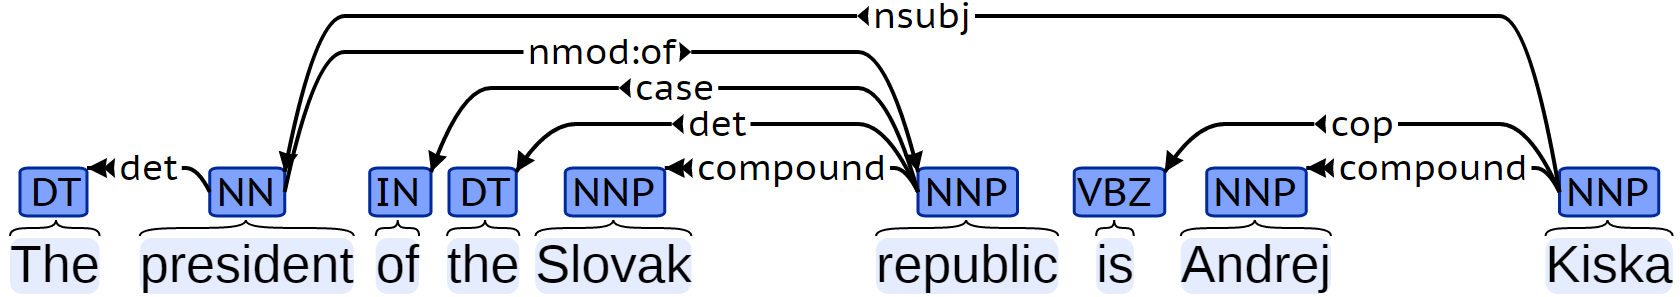
\includegraphics[scale=0.32]{example_sentence_andrej_kiska}\end{center}
	\caption[Zásivlostí jednoduchej vety]{Zásivlostí jednoduchej vety}\label{fig:example_sentence_andrej_kiska}
\end{figure}

\begin{figure}[H]
	\begin{center}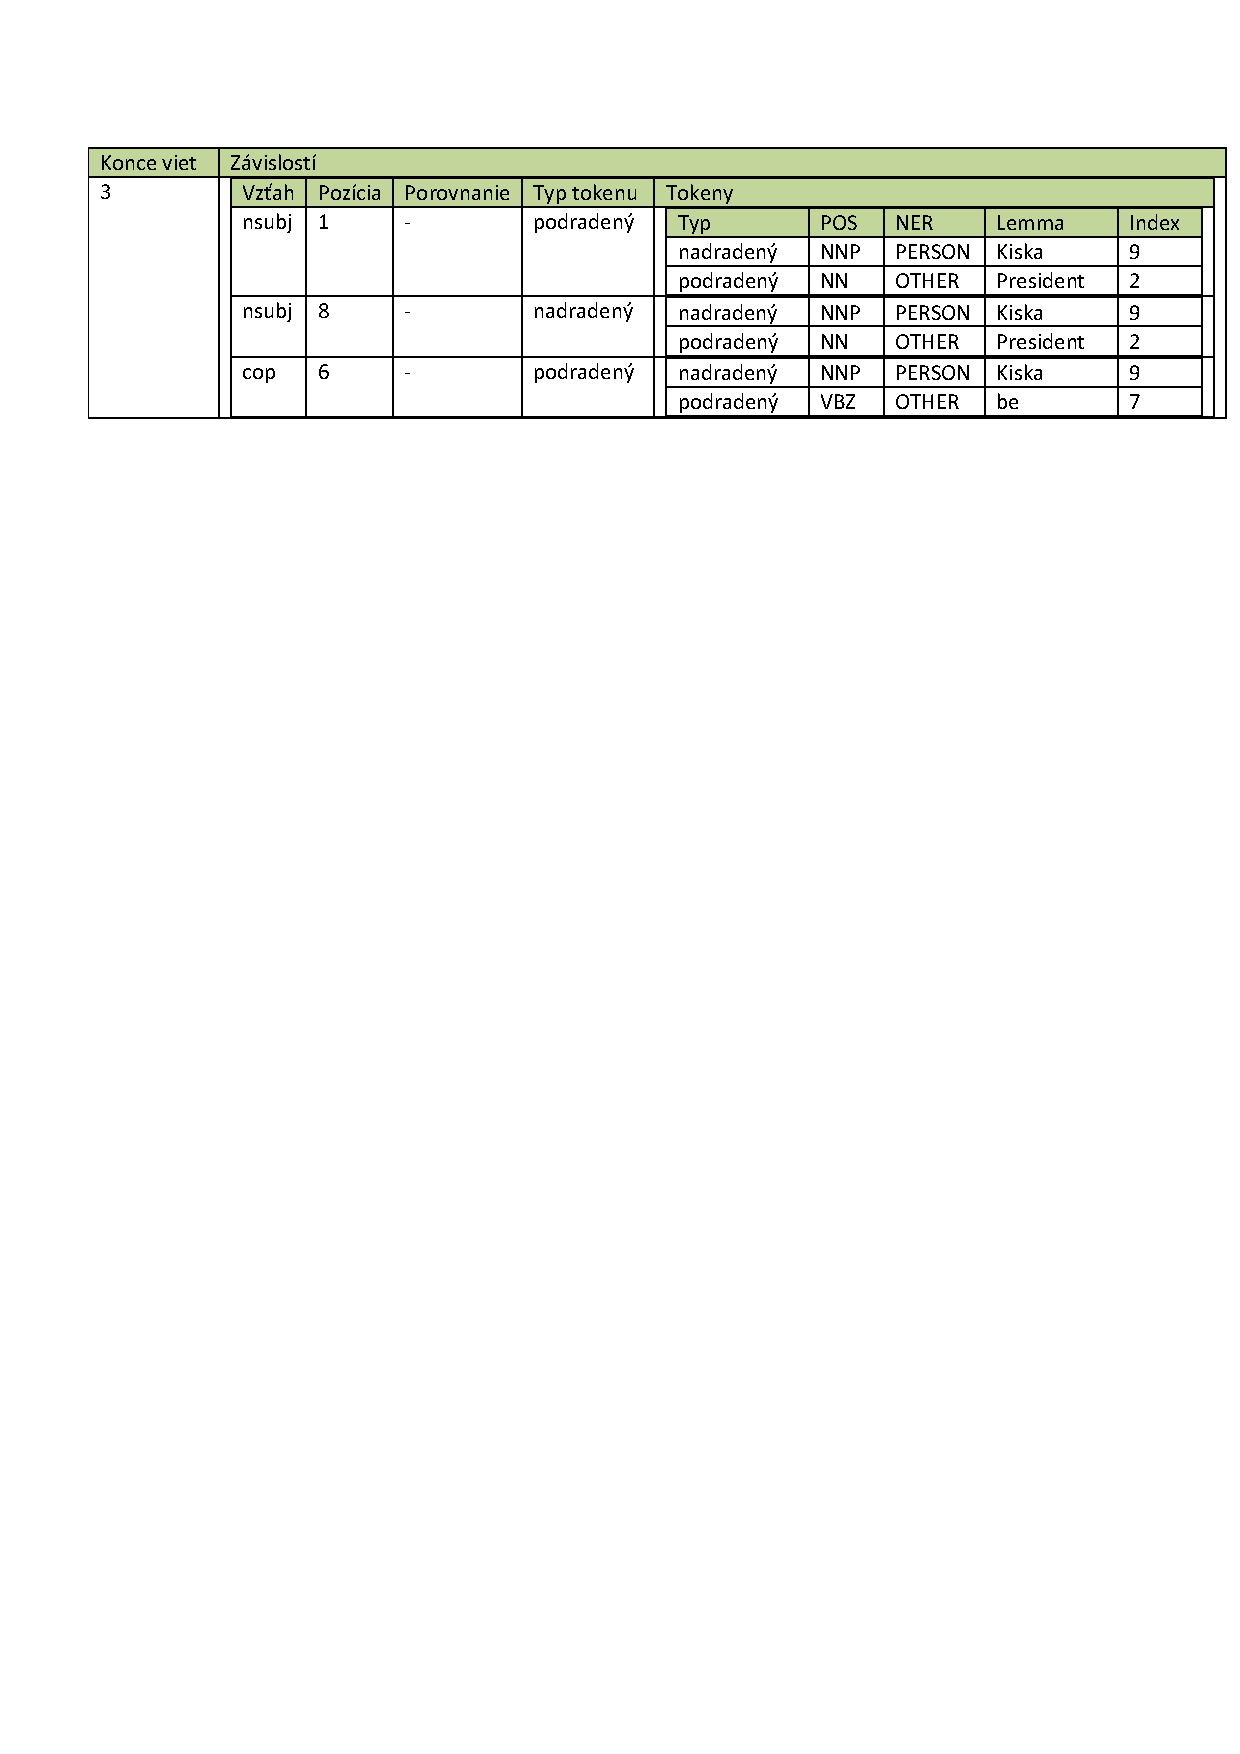
\includegraphics[scale=0.32]{apply_rule_example_rule}\end{center}
	\caption[Príklad pravidla]{Príklad pravidla}\label{fig:apply_rule_example_rule}
\end{figure}

%
% Výpočet zhody závislostí
%
\ifthenelse {\boolean{bachelor}}
{
	%\subsection{Subsection}
	\paragraph{Výpočet zhody závislostí}
}
{
	%\section{Subsection}
	\subsubsection{Výpočet zhody závislostí}
}
\label{paragraph:dependency_match}

Výpočet zhody závislostí pozostáva s niekoľkých krokov a princíp výpočtu je veľmi podobný s výpočtom zhody viet zo sekcie~\fullref{subsubsection:rule_lookup}. Porovnávajú sa vždy nadradené aj podradené tokeny. Porovnanie ma niekoľko krokov. Začína sa s porovnaním POS značiek. Pokračuje sa názvoslovnou entitou, indexom, lemou a nakoniec sa porovná vzdialenosť pozícií tokenov vo vetách. Každý krok je príslušne ohodnotený a ak porovnanie bolo úspešné, ohodnotenie sa pripočíta k finálnej hodnote reprezentujúca percentuálne zhodu závislostí.

%
% Vytváranie pravidla
%
\ifthenelse {\boolean{bachelor}}
{
	%\subsection{Subsection}
	\subsubsection{Vytvorenie pravidla}
}
{
	%\section{Subsection}
	\subsection{Vytvorenie pravidla}
}
\label{subsubsection:rule_creation}
Ak nám proces vyhľadania pravidla nevyhľadal žiadne pravidlo, znamená to, že sme doposiaľ nespracovávali takú istú alebo podobnú vetu. V tomto prípade sú použité statické pravidlá na spracovanie vety. Výstupom bude zjednodušená veta - poznámka.

Vytvorí sa záznam o pôvodnej vete, ktorý okrem iného obsahuje \textit{zoznam dát o pôvodnej vete}, ktorý sa vyskladá zo závislostí vety. Následne sa vytvorí záznam o pravidle, ktorý okrem iného obsahuje \textit{zoznam dát o poznámke}, vyskladaný zo závislosti poznámky. Nakoniec sa tieto dva záznamy prepoja a tým sa vytvorí nové pravidlo na spracovanie takej istej alebo podobnej vety, akú sme práve spracovali.

%Na obrázku~\fullref{fig:rule_creation} je znázornený proces nevyhľadania pravidla, použitia parsera s následným uložením nového pravidla.

%\begin{figure}[H]
%	\begin{center}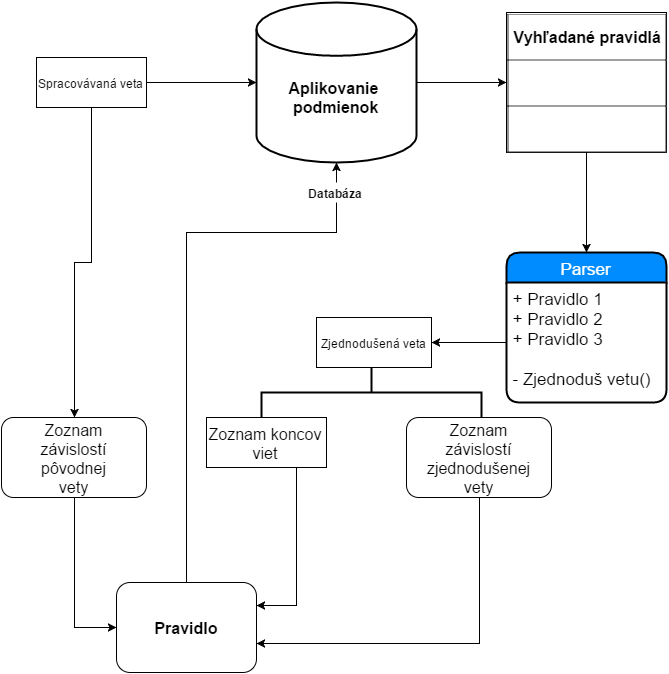
\includegraphics[scale=0.5]{rule_creation}\end{center}
%	\caption[Vytvorenie pravidla]{Vytvorenie pravidla}\label{fig:rule_creation}
%\end{figure}